\documentclass{article}
\usepackage{graphicx}
\usepackage{amsmath}
\usepackage{pgfplots}
\usepackage{physics}
\usepackage{cancel}
\usepackage{enumitem}
\usepackage{txfonts}

\pgfplotsset{compat=1.18}

\usepackage[a4paper, top=1cm, bottom=2cm, left=2cm, right=2cm, includehead, includefoot]{geometry}

\begin{document}

\noindent
Physics 4A - Classical Mechanics \hfill Prof. Roger King

\noindent\rule{\textwidth}{0.4pt}

\begin{center}
    \textbf{\LARGE Homework 7} \\
    \vspace{12pt}
    \large Aaron W. Tarajos \\
    \textit{\today}
\end{center}

\noindent\rule{\textwidth}{0.4pt}

\section*{Problem 1}
3.15-kg block is acted on by a 24.0-N force that acts at 37.0$^\circ$ below the horizontal, as
shown in the figure. Take $\mu_k = 0.200$ and $\mu_s = 0.500$. \\
(a) Does the block move if it is initially at rest? \\
(b) If it is initially moving to the right, what is the blocks acceleration?

\begin{figure}[ht]
    \centering
    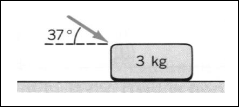
\includegraphics[scale=.5]{drawing-1.png}
\end{figure}

\subsection*{Solution}
\subsubsection*{Part a:}
Let $F_x$ be the horizontal component of the force vector $\vec{F}_1$ that is acting on the block given by;

\[
	F_x = F_1 \cos \theta
\]
If the block is at rest it will move when $F_x$ is greater than the force of static friction, $F_s$, acting on the block $F_x > F_s$ where $F_s$ is given by;

\[
	F_s = \mu_s F_n
\]
The normal force $F_n$ is given by

\[
	F_n = mg + F_1 \sin \theta
\]
So we have

\[
	F_x  = 24.00 \cos 37 = \boxed{19.167\ \text{N}}
\]
and

\[
	F_s = 0.500\left( 3.15 \cdot 9.81 + 24.00 \sin 37 \right) = \boxed{22.673\ \text{N}}
\]
Therefore, the block does not move if it is initally at rest.

\subsubsection*{Part b:}
If the block is moving to the right the acceleration is equal to the difference in the horizontal component of $\vec{F}_1$ and the force of kinetic friction,$F_k$ where;

\[
	F_k = \mu_k F_n = \mu_k \left( mg + F_1 \sin \theta \right)
\]
which gives us the equation

\[
	\vec{a} = \frac{F_1 \cos \theta - \mu_k \left( mg + F_1 \sin \theta \right)}{m}
\]
substituting our values;

\[
	\vec{a} = \frac{24.00 \cos 37 - 0.200\left(3.15 \cdot 9.81 + 24.00 \sin 37 \right)}{3.15} = \boxed{3.206\ \text{m}/\text{s}^2}
\]

\section*{Problem 2}
A block is released at the top of a 25$^\circ$ incline. Determine the coefficient of kinetic friction
given that it slides 2.30 m in 3.15 s.

\subsection*{Solution}
Given the distance traveled, $\Delta r = 2.30$, and the time, $t = 3.15$, we find the coefficient of kinetic frinction, $\mu_k$, by finding $\vec{a}$ as a function of $\mu_k$ and then solving for $\mu_k$ in the kinematic equation for distance.

\[
	\vec{a} = \frac{F_g - \mu_k F_n}{m}
\]
where $F_g$ is the force of gravity in the direction of the incline given by

\[
	F_g = mg \sin \theta
\]
and $F_n$ is the normal force that is opposing the force of gravity given by
\[
	F_n = mg \cos \theta
\]
Therefore, $\vec{a}$ is given by
\begin{align*}
	\vec{a} &= \frac{mg \sin \theta - \mu_k mg \cos \theta}{m} \\
		&= \frac{mg \left( \sin \theta - \mu_k\cos \theta \right)}{m} \\
		&= g\left( \sin \theta  - \mu_k \cos \theta \right)
\end{align*}
then the distance function becomes

\begin{align*}
	\Delta r &= v_0 t + \frac{1}{2}at^2 \\
	\Delta r &= (0) t + \frac{1}{2}\left( g\left( \sin \theta  - \mu_k \cos \theta \right) \right) t^2 \\
	\frac{2 \Delta r}{gt^2} &= \sin \theta - \mu_k \cos \theta \\
	\mu_k &= \tan \theta - \frac{2\Delta r}{gt^2\cos\theta}
\end{align*}
substituting the given values;

\[
	\mu_k = \tan25-\frac{2\cdot2.30}{9.81\cdot3.15^{2}\cos25} = \boxed{0.414}
\]

\section*{Problem 3}
A circular off ramp has a radius of 57.0 m and a posted speed limit of 50.0 km/h. If the
road is horizontal, what is the minimum coefficient of friction required?

\subsection*{Solution}
Centripital acceleration is given by

\[
	a = \frac{v^2}{r}
\]
therefore, centripital force is

\[
	F_c = m\frac{v^2}{r}
\]
The minimum coefficient of friction would be when $F$ is equal to $F_c$, otherwise the centripital force would overpower the friction force and the car would fall inward towards the center.

\begin{align*}
	F_c &= F_s \\
	m \frac{v^2}{r} &= \mu F_n \\
	m \frac{v^2}{r} &= \mu\ mg \\
	\mu &= \frac{v^2}{gr}
\end{align*}
Substituting the given values we find;

\[
	\mu = \frac{13.8889^2}{g 57.00} = \boxed{0.345}
\]

\section*{Problem 4}
A car travels at speed $v$ around a frictionless curve of radius $r$ that is banked at an angle to the horizontal. Show that the proper angle of banking is given by;
\[
	\tan \theta = \frac{v^2}{rg}
\]
(Hint, this is easier if you don’t rotate the coordinate system like most other incline problems, and treat the
x-axis as the horizontal direction, and the y-axis as the vertical direction. This is because the centripetal force is horizontal.)

\subsection*{Solution}
Consider the cross section of the banked curve, the forces acting on the car are.

\begin{center}
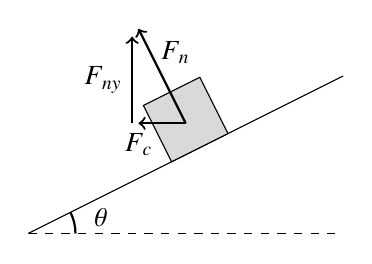
\begin{tikzpicture}[scale=0.40]
    % Points
    \coordinate (A) at (0,0);
    \coordinate (B) at (10,5);
    \coordinate (C) at (10,0);

    % Vectors
    \draw[-] (A) -- (B);
    \draw[-,dashed] (A) -- (C);

    \draw[fill=gray!30, rotate around={26.57:(5,2.5)}] (4.5,2.5) rectangle (6.5,4.5);

    \draw[->, thick] (5.0,3.5) -- ++(-1.5,3.0) node[pos=0.75, right] {$F_n$};
    \draw[->, thick] (5.0,3.5) -- ++(-1.5,0) node[left, below] {$F_{c}$};
    \draw[->, thick] (3.3,3.5) -- ++(0,2.75) node[pos=0.5, left] {$F_{ny}$};

    % Angle
    \draw [thick] (1.5,0) arc[start angle=0, end angle=26.57, radius=1.5];
    \node at (2.3,0.5) {\(\theta\)};

\end{tikzpicture}
\end{center}
Notice that
\begin{align*}
	\cos \theta &= \frac{F_{ny}}{F_n} \\
	F_n \cos \theta &= F_{ny} \\
	F_n \cos \theta &= mg \\
	F_n &= \frac{mg}{\cos\theta}
\end{align*}
and

\[
	F_c = F_n \sin\theta
\]
combining these two equations and using the equation for centripital force;
\begin{align*}
	F_c &= \left(\frac{mg}{\cos\theta}\right)\sin\theta \\
	m\frac{v^2}{r} &= \left(\frac{mg}{\cos\theta}\right)\sin\theta \\
	m\frac{v^2}{r} &= mg \tan \theta \\
	\tan\theta &= \frac{v^2}{rg}
\end{align*}

\section*{Problem 5}
A button is at the rim of a turntable of radius 15.0 cm rotating at 45.0 rpm. What is the
minimum coefficient of friction needed for it to stay on?

\subsection*{Solution}
The velocity is given by

\[
	v = \frac{2\pi r}{T}
\]
where $T$ is the period of revolution. Then the minimum friction coefficient is given by the equation derived in problem 3
\begin{align*}
	\mu_s &= \frac{v^2}{gr} \\
	      &= \left(\frac{2\pi r}{T}\right)^2 \cdot \frac{1}{gr}
\end{align*}
solving for the given variables;

\[
	\mu_s = \left(\frac{90\pi(0.15)}{60}\right)^{2}\cdot\frac{1}{(9.81)(0.15)} = \boxed{0.340}
\]

\section*{Problem 6}
A box is dropped onto a conveyor belt moving at 3.40 m/s. If the coefficient of friction
between the box and the belt is 0.270, how long will it take before the box moves without
slipping?

\subsection*{Solution}
We know that the force of static friction is given by

\[
	F_s = \mu_s mg
\]
and using Newton'n second law

\[
	m\vec{a} = \mu_s mg \implies \vec{a} = \mu_s g
\]
Then,

\[
	v = v_0 + at \implies t = \frac{v - v_0}{a}
\]
giving us the equation

\[
	t = \frac{v - v_0}{\mu_s g} = \frac{3.40 - 0}{(0.27)(9.81)} = \boxed{1.287\ \text{s}}
\]

\section*{Problem 7}
Two blocks are stacked as shown below, and rest on a frictionless surface. There is friction
between the two blocks with a coefficient of friction $\mu_s$. An external force is applied to the top
block at an angle $\theta$ with the horizontal. What is the maximum force $F$ that can be applied for
the two blocks to move together?

\begin{figure}[ht]
    \centering
    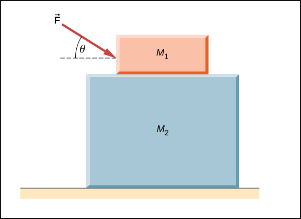
\includegraphics[scale=.5]{drawing-2.png}
\end{figure}

\subsection*{Solution}
The maximum force that can be applied for the two blocks to move together exists when the horizontal component of $F$ is equal to the static friction force that $m_2$ exerts on $m_1$.

\[
	F_s = F_x \implies \mu_s F_n = F\cos\theta
\]
where the normal force, $F_n$ is given by

\[
	F_n = m_1g + F\sin\theta
\]
Therefore the maximum force of $F$ is
\begin{align*}
	F\cos\theta &= \mu_s\left( m_1g + F\sin\theta \right) \\
	F\frac{cos\theta}{\mu_s} &= m_1g + F\sin\theta \\
	F\frac{\cos\theta}{\mu_s} - F\sin\theta &= m_1g \\
	F &= \frac{m_1g}{\frac{\cos\theta}{\mu_s} - \sin\theta} \\
\end{align*}
\[
	\boxed{F = m_1g \left(\frac{\mu_s}{\cos\theta} - \frac{1}{\sin\theta}\right)}
\]


\end{document}
